\section{Trabajo práctico integrador Nº 1}
\subsection{Selección del director de proyecto}
En el siguiente apartado se detallará el análisis y selección de la persona que ocupará el puesto de \textbf{director de proyecto}.
%Para ello se debe aplicar algún criterio de selección, con la justificación correspondiente.

\subsubsection{Análisis del puesto}
%Detalla cual es la necesidad por la que surge este puesto..después de una investigación exhaustiva se define qué tipo de posición se necesita en la organización y el alcance de la misma en cuanto a las necesidades presentes y futuras.

Se está iniciando un proyecto innovador de desarrollo de software enfocado en la salud.
En base a la definición de requerimientos ya concretada, se han detectado las siguientes necesidades: 
	\begin{itemize}
		\item Gestionar el esfuerzo de desarrollo, para lo cual es indispensable planificar qué tiempo va a llevar el mismo y su despliegue, qué recursos se van a necesitar, con qué capacidades y aptitudes se deben contar.
        \item Definir alcances y recursos a ser empleados en el proceso, para así estimar los costos fijos del mismo. 
        \item Monitorizar y controlar los avances y resultados.
        \item Evitar las confusiones presentes en la ``\textit{zona gris}'' entre especificaciones del usuario y el software a entregar.
        Es decir, se necesita de una persona concentrada en conectar estas especificaciones con los productos entregados, aplicando una metodología adecuada al tipo de proyecto y contexto actual de desarrollo de software.
        \item Contar con una persona que:
        \begin{itemize}
            \item Mantenga involucrado al usuario final, estableciendo una comunicación fluida y constante entre desarrolladores, clientes y usuarios.
            \item Tenga la capacidad para establecer objetivos realizables.
            \item Tenga gran experiencia en guiar la elaboración de requerimientos y especificaciones bien definidos y completos.
            \item Elabore, en el proceso, buenos reportes de estado.
            \item Pueda detectar y gestionar los riesgos.
            \item Aplique lo último en tecnología.
            \item Tenga habilidad para manejar el proyecto.
            \item Tenga sólidas prácticas de desarrollo, para apoyar al equipo en términos técnicos.
            \item Guíe los esfuerzos comerciales.
        \end{itemize}
	\end{itemize}
Por lo tanto, se necesita de un director de proyecto; una persona con una gran cantidad de capacidades y aptitudes, que tome el proyecto en el estado que se encuentra actualmente y lo dirija para alcanzar los objetivos planteados.


\subsubsection{Descripción del perfil requerido}

Este apartado detalla el trabajo que desempeñará el director de proyecto, y sirve como punto de partida en toda contratación y evaluación de desempeño.
La descripción del puesto inicia por trazar de forma general el puesto, para posteriormente detallar las responsabilidades, la línea de reporte, lugar de trabajo, rango de remuneración, horario y todo aspecto relacionado con una posición particular.

El \textbf{director de proyecto} es la persona que tiene la responsabilidad total del planeamiento y la ejecución acertados del proyecto.

Debe poseer una combinación de habilidades, incluyendo una gran capacidad inquisitiva y de resolver conflictos interpersonales.
Una de sus tareas más importantes es el reconocimiento de los riesgos que afectan directamente las probabilidades de éxito del proyecto, y la constante medición, formal e informalmente de dicho riesgo a lo largo del ciclo de vida del proyecto.
El director de proyecto acertado es aquel que enfoca esto como preocupación principal.
La mayor parte de los problemas que afectan un proyecto se relacionan de un modo u otro a un riesgo.

El director de proyecto es el responsable de tomar las decisiones necesarias de manera tal que el riesgo sea controlado y la incertidumbre reducida al mínimo.
Cada decisión tomada por él debe involucrar un beneficio directo hacia el proyecto.

\paragraph{Funciones}
            \begin{itemize}
                \item \textbf{Motivar}:
                Incentivar al equipo de trabajo para que aporte ideas y aumente su rendimiento, al hacer propio el objetivo del proyecto.
                
                \item \textbf{Toma de decisiones}:
                Decidir sobre el curso del proyecto, eligiendo entre las diferentes formas para resolver situaciones y conflictos que se presenten.
                
                \item \textbf{Comunicar}:
                Dar a conocer al equipo las decisiones tomadas y la planificación de tareas y estados de avance.
                
                \item \textbf{Administrar recursos}:
                Gestionar los recursos humanos, técnicos y económicos con el fin de lograr su máximo aprovechamiento y que sirvan para alcanzar el objetivo del proyecto.
                
                \item \textbf{Resolver y aprovechar conflictos}:
                Mediar ante los conflictos que se generen, buscando soluciones que impacten positivamente en los afectados y en el equipo de trabajo.
                
                \item \textbf{Planificar}:
                Determinar las tareas a llevar a cabo para concretar exitosamente el proyecto, administrando los recursos disponibles.
                Luego, programar y asignar las tareas resultantes.
                
                \item \textbf{Delegar tareas}:
                Traspasar la responsabilidad de llevar a cabo las tareas a los miembros del equipo.
                Sin embargo, la responsabilidad por la tarea no puede ser delegada, sólo el acto de realizar la tarea.
                
                \item \textbf{Organizar}:
                Detectar y posicionar cada recurso de la organización, para que cumpla la función específica que aportará a la consecución del proyecto.
                
                \item \textbf{Emitir órdenes e instrucciones}:
                Traspasar al equipo de trabajo no sólo las tareas a realizar, sino también los lineamientos que se deben cumplir al llevarse a cabo.
                
                \item \textbf{Liderazgo}:
                Llevar a cabo el ejercicio de la actividad ejecutiva del proyecto, y ser la figura encargada de la gestión y la motivación dentro del equipo de trabajo.
                
                \item \textbf{Negociar}:
                Buscar la satisfacción de necesidades del proyecto y de los miembros del equipo, al mediar entre intereses diferentes y tratando de conciliar conflictos.
                
                \item \textbf{Confeccionar y presentar reportes}:
                Brindar a la gerencia y al equipo de trabajo información relevante relacionada a la ejecución del proyecto, para detectar fallas en el proceso y/o motivar a los receptores de la misma.
                
                \item \textbf{Supervisar}:
                Controlar que se haya cumplido con la planificación, obteniendo una retroalimentación que pueda ser estudiada para mejorar el desarrollo del proyecto y el rendimiento del equipo de trabajo.
                
                \item \textbf{Ejercer coaching}:
                Acompañar en el proceso de aprendizaje, e instruir y entrenar al equipo de trabajo, con el objetivo de desarrollar en ellos habilidades que sean favorables para el desarrollo del proyecto.
                
                \item \textbf{Controlar cumplimiento}:
                Ejercer control sobre el trabajo del equipo, comparándolo con la planificación, para detectar demoras o dificultades.
                
                \item \textbf{Ejercer autoridad}:
                Llevar a cabo la función de mandar y dar órdenes, desde un nivel superior al equipo de trabajo.
            \end{itemize}
        
        
\paragraph{Responsabilidades}
            \begin{itemize}
                \item Identificar los requerimientos y el alcance del proyecto.
                \item Desarrollar el plan del proyecto.
                \item Dirigir, planificar y controlar el proyecto, dentro del presupuesto y los plazos de entrega fijados previamente por la empresa a que pertenece.
				\item Administrar los recursos humanos y materiales.
                \item Respaldar al equipo ante cualquier inconveniente durante el desarrollo del proyecto.
                \item Asegurar la funcionalidad y productividad del equipo.
                \item Coordinar y motivar el equipo de trabajo.
                \item Prever posibles desviaciones del proyecto; tener en mente el futuro próximo.
                \item Mediar en los conflictos interpersonales del equipo.
                \item Definir las características básicas del proyecto y controlar la asignación de tareas a las personas responsables, ya sea bajo su control directo o el de las unidades u organizaciones que intervengan.
                \item Organizar reuniones de planificación, trabajo y control.
                \item Administrar los costos, presupuesto y aseguramiento de la calidad.
                \item Dirigir, en los trabajos correspondientes al proyecto y con independencia de su situación en el organigrama, a las personas responsables de cada tarea adscrita al mismo.
                \item Exigir la calidad de los trabajos asignados, dentro de los presupuestos y plazos aceptados por los responsables directos de su ejecución.
                \item Identificar y controlar riesgos.
                \item Tomar las decisiones técnicas y económicas necesarias para el buen desarrollo de los trabajos.
			\end{itemize}
             
\paragraph{Perfil y capacidades}
            \begin{itemize}
                \item \textbf{Organización}:
                Distribuir eventos y actividades de acuerdo a los recursos y tiempos disponibles para llevar el proyecto al éxito.
                
                \item \textbf{Capacidad para planificar}:
                No sólo debe ser capaz de planificar, sino que debe interesarse especialmente por esta problemática.
                
                \item \textbf{Capacidad de juicio}:
                Debe ser capaz de compaginar las soluciones técnicas con los plazos, los costos y los factores humanos.
                
                \item \textbf{Capacidad de persuasión}:
                Encontrar y desarrollar argumentos para mejorar y ayudar en una situación.
                Contar además con buen carisma para las negociaciones.
                
                \item \textbf{Capacidad de abstracción}:
                Entender y comunicar aspectos no tangibles, como visión y misión del equipo de trabajo.
                Deberá, además, poder entender y ver el proyecto completo como una unidad y las relaciones entre sus partes.
                
                \item \textbf{Identificación de problemas}:
                Debe prever la existencia de problemas y tratarlos en la justa medida de su importancia.
                
                \item \textbf{Liderazgo y motivación}:
                La capacidad de motivar, el liderazgo, es el factor más importante del éxito.
                
                \item \textbf{Relaciones personales}:
                Facilidad para relacionarse con la gente, y buena comunicación oral y escrita.
                Permite desarrollar la confianza y la comunicación entre los involucrados del proyecto.
                Debe poseer una capacidad destacada para las relaciones personales.
                Es el representante principal del proyecto ante clientes, proveedores y otros stakeholders del proyecto.
                Además, debe dirigir a un conjunto de personas sobre los que normalmente no tiene poder jerárquico, y por lo tanto, es necesario hacerlo con grandes dosis de autoridad personal, tacto, habilidad y capacidad de convicción.
                
                \item \textbf{Capacidad de adaptación}:
                Debe de ser muy flexible, capaz de adaptarse a muchas y cambiantes circunstancias.
                
                \item \textbf{Técnico}:
                el dominio de la tecnología principal del proyecto es el punto de partida necesario para que el Jefe de Proyecto pueda comprender los puntos clave del mismo, planificar los recursos, generar ideas y soluciones eficaces, controlar la calidad, etc.
                                
                \item \textbf{Poder de concretización}:
                utilizando los recursos e información disponibles, obtener conclusiones y tomar acciones específicas para manejar el proyecto.
                                
                \item \textbf{Experiencia}:
                Haber estado al mando de proyectos con anterioridad, sean o no de la misma naturaleza que el proyecto actual.
                
                \item \textbf{Creatividad}:
                Sin dejar de ser realista, encontrar y proponer soluciones creativas a los problemas o conflictos que se presenten, tomando decisiones y ejecutando acciones cuando el plan actual no funciona.
                Resuelve actividades complejas e interdependientes convirtiéndolas en tareas más pequeñas que se documentan.
                La creatividad recae en que no aplica la misma solución a diferentes problemas.
                
                \item \textbf{Gestor}:
                Poseer una notable aptitud gestora, pues no sólo se encarga de una dimensión técnica, sino que debe controlar y conseguir todos los objetivos del proyecto, incluyendo los financieros y de plazo, que suelen ser los más críticos y con mayor frecuencia incumplidos.
			\end{itemize}



\paragraph{Descripción del candidato}

%Una vez que se conoce qué tipo de posición se necesita cubrir, y la forma en la que ésta impactará a la organización, se describe a la persona ideal y se es muy específico en describir las habilidades, conocimientos, aptitudes y experiencia que requiere el candidato, así como el dominio de idiomas y nivel de estudios, entre muchos otros requisitos.

En base al análisis del puesto de ``director de proyecto'', junto con la descripción del perfil requerido, y atendiendo a las funciones, responsabilidades y capacidades del mismo, se ha propuesto a \textbf{Michael Manganiello} como director de proyecto.
La decisión se basa en las aptitudes y habilidades técnicas, personales, interpersonales y de liderazgo y motivación, entre las cuales se destacan las siguientes:

\begin{itemize}
    \item Capacidad de resolución de conflictos.
    \item Seguridad en el tratamiento de temas técnicos.
    \item Iniciativa ante el surgimiento de problemas.
    \item Experiencia en diferentes ámbitos técnicos, que proporciona una visión global.
    \item Creatividad para la propuesta de soluciones a problemas y conflictos.
    \item Serenidad y templanza, en los momentos en que se requiere el detenimiento al pensar y contemplar las posibilidades del equipo.
    \item Control de emociones, para gestionar situaciones que así lo requieran dentro y entre miembros del equipo, y con personas ajenas al mismo.
    \item Focalización en objetivos, lo que no sólo se torna en una capacidad proactiva, sino que es motivadora para el resto de los integrantes.
\end{itemize}

\newpage

\subsection{Estilos de liderazgo y resolución de conflictos}
El Director deberá decidir y registrar qué estilo de liderazgo utilizará y el enfoque de resolución de conflictos que aplicará en supuestas situaciones (que también detallará) que se le puedan presentar durante el proyecto.

\subsubsection{Estilos de liderazgo}

A continuación se describen los diferentes estilos de liderazgo:

\begin{itemize}
\item\textbf{Líder liberal o líder \textit{Laissez faire}}:
\textit{Laissez faire} es una expresión francesa que significa ``dejen hacer'' o ``dejen pasar''.
De ahí, que este estilo de liderazgo se caracterice por una libertad completa por parte del grupo en las decisiones y una participación mínima del líder.
El líder no ejerce su función, no se responsabiliza del grupo y deja a éste a su propia iniciativa.

\item\textbf{Líder democrático}:
Las directrices son debatidas por el grupo y decididas por éste, con el estímulo y apoyo del líder.
Se basa en la colaboración y participación de todos los miembros del grupo.
El líder y los subordinados actúan como una unidad.

\item\textbf{Líder autocrático}:
El líder fija las directrices sin participación del grupo.
El líder concentra todo el poder y la toma de decisiones.
Es un ejercicio de liderazgo unidireccional; lo único que tienen que hacer los subordinados es obedecer las directrices que marca el líder.
\end{itemize}

\subsubsection{Elección del estilo de liderazgo}

Teniendo en cuenta las definiciones anteriores y la forma de trabajar de nuestra empresa de desarrollo, se considera que el estilo de liderazgo que deberá preponderar en el director es el de \textbf{líder libre}, ya que con el tiempo se ha logrado mantener a los miembros del equipo y como consecuencia la confianza entre los mismos ha crecido considerablemente.
Debido al tiempo de iniciado del proyecto, se tiene en cuenta que el director puede no tener todos los conocimientos que son necesarios, por lo que muchas veces el director puede no estar preparado para tomar decisiones, y todo dependerá de las decisiones que toma el equipo.
De todos modos, se sabe que el manejo del proyecto depende totalmente de las situaciones que se presenten, por lo que en ocasiones se aceptará la toma de decisiones del director según un estilo democrático o autocrático.
De acuerdo a este estilo de liderazgo preponderante, se entiende que el enfoque que seguirá la resolución de conflictos por lo general será de \textbf{carácter colaborativo y de arreglo}, aunque en algunas situaciones sabemos que los enfoques agresivo, evasivo y acomodaticio representarán la mejor opción y serán tenidos en cuenta. 


\subsubsection{Consideración de conflictos}

%Se me ocurren las siguientes. 
A continuación, se especifican una serie de conflictos que podrían presentarse durante la ejecución del proyecto:

\begin{itemize}

\item \textit{Un desarrollador inexperto no sabe cómo resolver un problema que requiere conocimientos de patrones de diseño de software}:

El director consulta al líder técnico, y éste demuestra gran capacidad para resolver el conflicto.
Luego, para evitar futuros conflictos y seguir el enfoque de colaboración, el director reúne al conjunto de desarrolladores inexpertos con el líder técnico y resuelven el conflicto de forma colaborativa y con el objetivo de aprender y evitar que el conflicto se repita en el futuro, manteniendo el aprendizaje en la base de conocimiento del equipo.

\item \textit{El cliente plantea que el tiempo de entrega de la primera versión se ha adelantado}:

Siguiendo un enfoque de \textbf{arreglo}, el director propone al equipo que realicen horas extras para lograr los objetivos actuales, con la promesa de que una vez pasada la fecha de entrega se permitirá a los integrantes del equipo tomar un día de descanso en el momento que ellos lo decidan.

\item \textit{Un desarrollador resuelve un problema de diseño que no esté de acuerdo con consideraciones de cohesión y acoplamiento}:

Siguiendo un enfoque \textbf{agresivo}, podría aceptarse esta solución rápida y continuar con el desarrollo.
Sin embargo, según el enfoque de arreglo, esta solución genera inconsistencias o errores futuros, por lo que la decisión del director debería ser la de frenar la actividad de diseño y continuarla en conjunto con alguien que posea los conocimientos para resolver el problema de forma correcta en cuanto a estas cuestiones esenciales en la etapa de desarrollo.

\item \textit{El desarrollador no recibe suficiente descripción o claridad acerca de los defectos por parte del tester}:

Este conflicto genera que los arreglos que realiza el desarrollador pueden no llegar a ser los adecuados.
Por esto, se define una plantilla que debe seguir el tester, la cual funciona como respaldo cuando los pedidos de colaboración no dan resultado.

\item \textit{Pobre comunicación entre los participantes sin alguna razón aparente}:

El director tendrá que entrar en acción y lograr que se entienda que para la concreción del proyecto es importante que los integrantes se comuniquen más allá de sus diferencias, por sus propias personalidades o por cualquier tipo de conflicto que tengan entre ellos.
El director debe identificar estas situaciones y tomar un enfoque de \textbf{arreglo} y \textbf{agresivo}, en el que va a dar las instrucciones y guiará la comunicación sin olvidar de seguir cada uno de los acontecimientos.

\item \textit{Uno de los participantes no realiza su parte del trabajo}:

Puede ocurrir que por diversos motivos (personal, laboral u otros), uno de los participantes del proyecto no esté llevando adelante las tareas que le corresponden.
En este tipo de casos, el director deberá intervenir tomando un enfoque de \textbf{colaboración}, preguntando qué sucede, por qué no realizó el trabajo asignado, tratando de solucionar posibles conflictos y poniéndose a disposición de sus liderados.

\item \textit{Reuniones poco eficaces}:

Ocurre muchas veces, que en las reuniones de trabajo no se avanza tanto como se espera.
Esto puede ser por distracción, no muy buena planificación de las tareas y tiempos que llevará cada una.
En estos casos, el director deberá estructurar las reuniones de forma tal que no deje lugar a la distracción y se aproveche en un 100\% el tiempo para las actividades que deben ser previamente planificadas.
Se recomienda que el director actúe preguntando a cada miembro qué se puede hacer, qué actividades se pueden llevar adelante y los tiempos estimados para las mismas.
También es de utilidad definir moderadores que cambien con el tiempo y apoyen en el objetivo de hacer reuniones útiles tanto para los participantes como para el proyecto.

\item \textit{Poca motivación de los miembros}:

Puede ocurrir que algunos miembros del grupo se encuentren desanimados.
Esto puede deberse a situaciones personales; puede que no estén a gusto con la actividad que realizan o con el mismo proyecto.
El director puede asumir un enfoque de \textbf{colaboración} y percibir las inquietudes, proponer mejoras motivacionales para llegar a un consenso y obtener así compromiso de parte de los participantes, haciéndolos sentir una parte fundamental del equipo.

\item \textit{Falta de conocimientos del equipo}:

Este es el caso en el que algunos integrantes dominen, mejor que otros, determinadas herramientas, o demuestren mayores capacidades para resolver tareas en menos tiempo y con mejores resultados.
Esto puede generar inconvenientes porque algunos trabajan más y obtienen mayor cantidad de resultados que otros.
En este tipo de casos, el líder del equipo debe tomar un enfoque \textbf{colaborativo}, capacitando a aquellos que lo requieran, y de \textbf{arreglo}, al brindar beneficios a aquellos con conocimientos y que dediquen tiempo a compartir y enseñar a los demás.
El director debe dar apoyo, acompañamiento y disolver los sentimientos que han interferido en la relación de los participantes.

% \item Otros conflictos que se pueden presentar son si cambian los requisitos, la distribución de actividades técnicas, el grado de interacción entre clientes y desarrolladores

\end{itemize}

\begin{comment}
El estilo es la forma en que va a ejercer cualquiera de los 4 tipos de liderazgo
* Libre: Usado cuando hay mucha confianza en el equipo o cuando son actividades en las que el líder no se encuentra preparado. Se brindan lineamiento para planificar actividades y luego se evalúan los entregables. El control y supervisión diario es menor a los otros tipos
* Autocrático: Poca participacion.
* Participativo: Se dedica al personal participando continuamente en las opiniones, escuchando y guiando al equipo. Existe una gran supervisión
\end{comment}

\newpage

\subsection{Técnicas de motivación}

\subsubsection{Introducción}

El Director debe registrar al menos 5 técnicas de motivación que utilizará durante el proyecto, si fuera necesario, y detallar en qué tipos de situaciones sería necesario aplicar cada una.

\subsubsection{Tipos de motivación}

Las técnicas de motivación que el líder llevará a cabo van a depender del tipo de situación en el que el se encuentre con respecto a las necesidades o los deseos de las  personas a las que se va  a dirigir. Estas necesidades de los empleados pueden observarse en una escala a través de la pirámide de Maslow que se muestra en la \textbf{Figura \ref{Maslow}}.
 \begin{figure}[h]
  \centering
  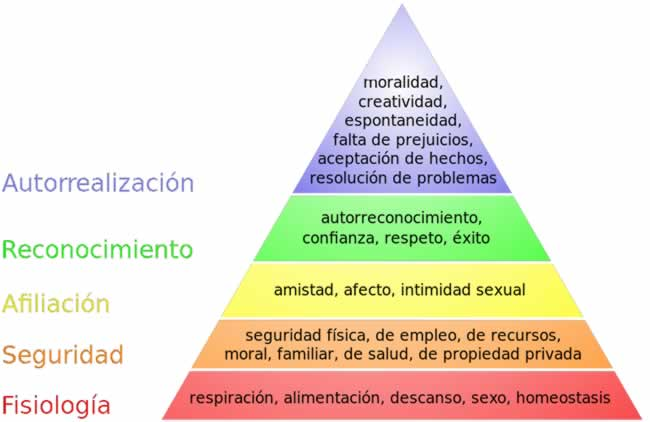
\includegraphics[width=.8\textwidth]{img/tp1_integrador/piramide_de_maslow}
  \caption{Pirámide de Maslow}
  \label{Maslow}
\end{figure}
\begin{quote}
\small "Si queremos motivar a las personas que tenemos a nuestro alrededor debemos buscar que necesidades tienen satisfechas e intentar facilitar la consecución del escalón inmediatamente superior" 

Abraham Maslow
\end{quote}
Existen dos técnicas generales que permiten motivar el esfuerzo y provocar que el rendimiento laboral mejore. Ambas técnicas se encuentran muy relacionadas con las necesidades antes mencionadas y se detallan a continuación:
\begin{itemize}
\item \textbf{Técnicas de motivación positivas}: 
Estas técnicas permiten lograr, en un comienzo, un incremento pequeño en la productividad de los individuos pero que será sostenido a lo largo del tiempo.
\item \textbf{Técnicas de motivación negativas}: 
Estas técnicas producen que en un comienzo el rendimiento laboral crezca rápidamente pero que luego comience a disminuir con el paso del tiempo, teniendo que volver a realizar incentivos para lograr el rendimiento deseado. 
\end{itemize}

Existen 6 motivos por los que una persona  puede sentirse motivada y son estos sobre los que el director debe hacer hincapié para lograr un resultado destacables utilizando diversas técnicas específicas:
\begin{enumerate}
\item \textbf{Frente a lo nuevo}: Se refiere al impulso que sienten algunas personas de superar retos y obstáculos para alcanzar metas. El director debe detectar a estas personas para asignarle aquellas tareas que requieran un gran esfuerzo y recompensarlo en igual medida que la dificultad a las que se los expuso.

\item \textbf{Por poder}: Es un impulso por influir en los demás y modificar situaciones. Las personas motivadas por el poder desean causar un impacto en su organización y están dispuestas a correr riesgos para lograrlo. El director debe asignarle a las personas con este tipo de necesidades de motivación cargos de tipo gerenciales en los que puedan influir en el comportamiento de otros para el bien de la organización.

\item \textbf{Por prestigio}: Referido a aquellas personas que sienten una gran necesidad por obtener reputación , renombre y fama.  Estas demuestran su necesidad de sentir prestigio a través del deseo de sobresalir, necesidad de llamar la atención o afán de ser importante.
Por este motivo es necesario que el Director detecte quienes son estas personas y cuales son las cualidades que debe destacar para aumentar su prestigio en la empresa.  
Una técnica de motivación en este caso consiste en reconocer sus buenos desempeños, objetivos, resultados o logros obtenidos. Para ello puede recompensar económicamente sus buenos desempeños, elogiarlos por el trabajo realizado, o darles reconocimiento ante sus compañeros, por ejemplo, a través de una ceremonia en donde se premie a los empleados que mejor desempeño hayan tenido en un periodo de tiempo.

\item \textbf{Por altruismo (intrínseca)}: Una persona animada por motivos altruistas trabaja hasta que ha satisfecho las necesidades del otro.
La motivación para el empleado es superar sus propios intereses por el bien del equipo y la organización.
Una técnica importante de la que debe hacer uso el Director es involucrar a estos tipos de empleados en proyectos de gran valor para la empresa, para que sientan que su trabajo es vital para el correcto funcionamiento de la compañía.

\item \textbf{Adquisitiva (extrínseca)}: aparece cuando lo que atrae al individuo no es la acción que se realiza en sí, sino lo que se recibe a cambio de la actividad realizada (por ejemplo, una situación social, dinero, comida o cualquier otra forma de recompensa).
Para este caso es necesario que el líder brinde recompensas, tangibles o intangibles, a este tipo de empleados. Ejemplos de Recompensa tangible son pagos, promociones o castigos. Ejemplos de intangibles son alabanzas o elogios en público.

\item \textbf{Afiliación}: Relacionado a aquellas personas que tienen la necesidad de experimentar la sensación de pertenencia y de tener un elemento de identidad que contribuya a un cierto grado de seguridad y le permite buscar la aceptación y aprobación del grupo en el que se desenvuelve. 
En este caso es importante que el director introduzca a aquellos empleados con estas necesidad en un grupo donde el compañerismo prevalezca sobre las demás  características y donde se realicen actividades concurrentes en las que se les fomente el sentido de pertenencia.
También es necesario que el líder muestre interés por sus acciones, logros o problemas; no sólo por lo que suceda dentro del ámbito de la empresa, sino también, por lo que pueda suceder en su vida personal.
Para ello el director podría preguntarles y aconsejarlos sobre sus problemas personales, apoyarlos en sus metas personales o de desarrollo, por ejemplo, dándoles tiempo y permiso para que lleven estudios, o incluso financiar parte de éstos.
\end{enumerate}
% http://candelaramirezalmarosa.blogspot.com.ar/2008/02/114las-necesidades-humanas-como.html
% http://motivacionempresa.galeon.com/productos2280387.html
% http://morasolano.tripod.com/id13.html
\begin{comment}
Enfoque que le da el director de proeyecto a las tareas de acuerdo a las necesidades
El lider debe detectar cual es el puesto numero 1 para cada uno de las personas
Con la motivacion perseguimos mejorar el rendimiento laboral

Piramide de maslou

Autorealización
Auto estima
Afecto
Seguridad
Basicas
El lider debe conocer de cada persona cuales son sus fines. También debe conocer cuales son sus valores
Existen técnicas de motivación positivas  y técnicas negativas para mejorar el rendimiento laboral. Las técnicas negativas a lo largo del tiempo produce que el rendimiento laboral se mantenga y disminuya.  La  positiva logra un incremento pequeño pero sostenido en el tiempo, muy relacionado a como estén las necesidades en la piramide.

Un ejemplo de Motivación positiva es el caso de dar a conocer lo importante que es el trabajo de las personas ya sea de forma pública o no. 
Las tecnologías negativas producen ausencia de insatisfacción.
Las tecnologías positivas producen satisfacción.Estilo de liderazgo, forma de ejercer cualquiera de los cuatro tipos de líder. Puede ser libre (cuando el equipo tiene mucha capacidad, hay confianza, pueden tomar decisiones. En este se dan lineamientos y se miran entregables), autocrático (no se tiene todos los conocimientos que maneja el equipo) y participativo (es el que lleva más tiempo).
¿Por que motivar?
1. Frente a lo nuevo: nuevos desafios, por herramientas, etc
2. Por poder: 
3. Por prestigio: reconocimiento público, es recomendable felicitarlo frente a los otros, teniendo en cta aquellos que se deprimen.  
4. Por Altruismo: sentirse útil ante los demas
5. Adquisitva: Incorpar elemento.
6. Por pertenecer: estar en un grupo de compañeros
___________________________________________________________
Motivación, pirámide de maslow, le agrega escala de valores/ranking de necesidades. La misión del líder tiene que encontrar qué es lo principal para cada persona. Con la motivación se busca mejorar el rendimiento laboral. Existen técnicas de motivación + y -, esto se basa en que en el tiempo, si el rendimiento laboral viene constante la hace crecer un tiempo y vuelve a caer . La positiva un aumento de la productividad pequeño pero sostenidos en el tiempo (incorporarlas a tomar decisiones, capacitación, hacerle ver la importancia de lo que realiza en el proyecto por más mínima que sea). Por qué se motiva la gente? cinco formas de motivar: 
1. frente a lo nuevo, 
2. por poder (sobre cosas, personas), 
3. por prestigio (reconocimiento público), 
4. altruística (se motiva por el solo hecho de sentirse útil para los demás),
5. adquisitiva (monetaria, equipo, apuntes), 
6. afiliación (solo por el hecho de pertenecer). 
Negativa (ausencia de insatisfacción), positiva (genera satisfacción)
\end{comment}

\newpage

\subsection{Riesgos del proyecto}

\subsubsection{Introducción}
Se debe consensuar entre el equipo y su Director de Proyecto qué riesgos pueden aparecer en el proyecto y qué impacto tendrían sus consecuencias. También detallará cuáles son las medidas preventivas para cada uno de los riesgos. Recordamos que las medidas preventivas tienen como objetivo reducir la probabilidad de ocurrencia de cada riesgo o reducir el impacto que produciría cada riesgo.

\subsubsection{Riesgos detectados}
Después de consensuar con el equipo se dejan en claro los diferentes riesgos que podrían aparecer, su impacto tanto en el proyecto como en el equipo y sus acciones preventivas.

\begin{enumerate}
\item \textit{Abandono por parte de uno de los integrantes del grupo}:

La posibilidad de que algún integrante abandone ,ya sea por problemas de índole personal o laboral, en cierta medida es muy baja, pero si se concreta la repercusión en el grupo influirá de manera notable ya que en el equipo existe una planificación establecida con tareas y funciones previamente establecidas para desarrollar el proyecto. Algunas medidas que puedan llegar a evitar esto o disminuir el impacto, serían reuniones personales por parte del director con cada integrante de manera de detectar sus necesidades y brindarle diferentes soluciones, o al menos nos permitiría prever un posible abandono para salir a la búsqueda de un reemplazante e iniciar su capacitación para reemplazarlo.

\item \textit{Falta de documentación de las tecnologías a utilizar}:

Existe la posibilidad que la tecnología seleccionada no posea buena calidad de documentación (cuestiones sobre como resolver problemas o de como implementarla) y sea necesario hacer un análisis de las soluciones por nuestros propios medios. Esto provocaría atrasos en el desarrollo o en diferentes actividades del Devops (Persona dedicada al desarrollo y despliegue de la infraestructura), corriendo el riesgo de no poder terminar con el proyecto a tiempo. Se podría evitar, realizando un relevamiento detallado de las tecnologías a utilizar para tomar una buena decisión a la hora de seleccionarla. Otra solución para mitigar este riesgo sería contactarnos con personas que conozcan la tecnología y sean capaces de ayudarnos con los temas necesarios.

\item \textit{Dificultad de aprendizaje de la tecnología a utilizar}:

Los integrantes del proyecto tiene experiencia en programación pero para mejor el desarrollo se utilizarán herramientas nuevas que requerirán un período de adaptación a la misma, es por eso que se diagramó un plan de capacitación con cierta cantidad de horas cuyo principal riesgo es que no sea suficiente este tiempo para poder asimilar bien la tecnología y el conocimiento transmitido. Es posible que a algunos integrantes les sea suficiente pero hay una alta probabilidad de que no todos maduren el conocimiento de la misma manera como consecuencia de poseer diferentes capacidades de aprendizaje. Esto traería como consecuencia el atraso en el proyecto y horas sobrecargadas o un detrimento en la calidad del sistema a desarrollar. Algunas medidas preventivas podrían ser reunir al grupo y  elaborar un panorama con las diferentes dificultades a tener en cuenta de manera de sobrecargar con más horas a quien necesite más tiempo de capacitación. Otra forma de disminuir el impacto de dificultad de aprendizaje es realizar cursos que traten sobre las tecnologías a utilizar.

\item \textit{Pérdida del soporte o compatibilidad hacia atrás de la tecnología que se está utilizando}:

Suele suceder que ciertas tecnologías son actualizadas y deja de haber soporte para la versión que se está utilizando, esto produce, en el caso de los frameworks, que muchas  tareas que antes se realizaban automáticamente por el mismo, ahora necesiten mayor atención por parte del desarrollador. Otro caso se produce con las librerías que pierden soporte y produce que la aplicación se atrase con respecto a las tendencias y funciones mas utilizadas. Ambas situaciones provocan retrasos en el proyecto incrementando los costos. Una medida preventiva sería elegir una tecnología instaurada,  de software libre, que garantice el mantenimiento gracias a la gran comunidad que lo respalda.

\item \textit{Problemas de configuración de entornos de desarrollo y pruebas}.

Es común que en la configuración de  entornos de desarrollo surjan problemas con las diferentes versiones y valores establecidos para dicha configuración. Se nos presenta como riesgo ya que es un tiempo considerable que se puede invertir en otra etapa y como se explicó en el riesgo anterior en el atraso de las tareas, se ve influenciado todo el proyecto, teniendo el riesgo de no llegar a tiempo con las entregas programadas. Una medida para evitar este problema sería encargar a cada uno de los miembros a aprender de fondo un tema y de este modo contar con una persona que comprenda el entorno de desarrollo y sea capaz de documentar en una "wiki" los pasos necesarios a seguir, para que todo el grupo sea capaz de llevarlo a cabo.

\item \textit{Cambio de políticas o leyes gubernamentales que afecten a la organización y a su vez a nuestro sistema}:

El sistema se encuentra íntimamente relacionado con la información personal y por este motivo se encuentra sujeta a las modificaciones que hayan a nivel legal con respecto al manejo de datos personales. Actualmente  la Ley 26.529 establece los derechos del paciente referido a la documentación e información clínica y a la relación con los profesionales e instituciones de salud, si se produciera algún cambio sobre está ley nos afectaría directamente y tendríamos que re-analizar la situación.

Una medida a considerar pueden ser mantener un acuerdo directo con el usuario, para que futuros cambios en el ámbito legal no nos afecte en forma directa.

\item \textit{Aparición o detección de nuevos requerimientos}:

Idealmente, luego de la etapa de Análisis, no deberían aparecer nuevos requerimientos. Sin embargo  la experiencia nos ha enseñado que no siempre es así. Este es un riesgo a tener en cuenta ya que si aparece un nuevo requerimiento en una etapa avanzada del proyecto es muy probable que se retrasen otras tareas o modifiquen ciertos elementos ya cerrados que se verán afectados por los mismos. Las medidas preventivas que se pueden establecer son realizar un análisis exhaustivo de las necesidades del mercado y desarrollar el sistema utilizando buenas prácticas de diseño para desacoplar las funcionalidades y así lograr la máxima independencia entre ellas.

\item \textit{Adelanto de la fecha de entrega}:

Puede darse la situación de que sea necesario entregar el sistema antes de lo previsto por que surge alguna oferta importante de un cliente, lo que provocaría agilizar los tiempo, (contratando a mas personal y por ende aumentando los costos) o recortar funcionalidades. Una medida a considerar sería  realizar una correcta planificación indicando los sprints correspondientes que se llevarían a cabo en cada fecha determinada, para de este modo poder ofrecer de forma correcta cuales son las funciones a entregar en cada una de las fecha correspondientes, siempre teniendo en cuenta la integridad del sistema.
\end{enumerate}
\begin{comment}
Plan de contingencia != “tener previsto q hacer- tiene q incorporrse a la planificacion”
Riesgo deriva hacia el impacto. Los riesgos de los que hablamos son exclusivos del proyecto. Existen dos consecuencias a destacar. 
Demoras 
Mayores costos.
Lo preventivo tiene como objetivo reducir el impacto o la probabilidad de ocurrencia.
Medidas preventivas: reducen el impacto, o reducen la probabilidad de ocurrencia
Impacto: capacitación previa de programación para reducir las demoras del hecho de q solo 1 programe
Probabilidad de ocurrencia
Las medidas preventivas deben estar en el diagrama de gantt (planificación)
________________________________________________________________________
Riesgos del proyecto y su impacto. No es general como un plan de seguridad o contingencia, exclusivamente del proyecto. Debemos considerar que los riesgos generan dos consecuencias, demoras o mayores costos.
De c/ riesgo sus medidas preventivas las cuales reducen el impacto o la probabilidad de ocurrencia. Incorporar medidas preventivas a la planificación del proyecto.
\end{comment}

\newpage

\subsection{Método y actividades para la conversión del sistema}

\subsubsection{Introducción}

Se debe consensuar entre el equipo y su Director de Proyecto cuál será el método de conversión del Sistema (para pasar del sistema actual al nuevo), con todas las actividades a realizar. Se debe registrar en este punto no sólo el método y las actividades sino también la justificación correspondiente al máximo nivel de detalle

\subsubsection{Métodos de conversión de sistemas}

Nuestro sistema se encuentra orientado al paciente principalmente a aquellos que llevan sus análisis de forma física en carpetas almacenadas en algún lugar de su casa, lo que nosotros buscamos es brindarle un sistema totalmente diferente al sistema que usa actualmente, brindándole la posibilidad de gestionar no solo sus análisis sino también su información general de salud.

No se pretende eliminar el sistema de historia clínica que actualmente usan los centros de salud, pero si se encuentra en nuestros planes que las personas puedan utilizar este sistema como medio de comunicación con el médico.

Somos conscientes que lograr que los pacientes utilicen este sistema será un gran desafío, pero para esto se armará un plan de conversión estratégico detallando los métodos y actividades necesarios para la conversión junto con la justificación correspondiente.

Actualmente  existen 5 métodos de conversión de sistema:
\begin{itemize}
\item Conversión directa.
\item Conversión paralela.
\item Conversión gradual o por fases.
\item Conversión de prototipo modular.
\item Conversión distribuida.
\end{itemize}

\subsubsection{Elección de método de conversión}

Se usará el método de \textbf{conversión paralela} ya que nuestro sistema convivirá con la forma de gestión que posea el usuario, permitiéndole la posibilidad  de comparar las ventajas y detectar los beneficios que brinda el nuevo sistema.
Además este método está recomendado para aquellos casos en los que un sistema computarizado remplaza uno manual y es lo que pretendemos hacer en nuestro proyecto.

\subsubsection{Descripción de actividades para la conversión}

A continuación se describirán todas las actividades que se llevarán a cabo para implementar el nuevo sistema. Se identificará a todas las personas responsables de cada actividad  y el tiempo correspondiente a cada una
\begin{enumerate}
\item \textbf{Preparación de datos y archivos}:

Será necesario determinar cuál será la base de conocimiento que se cargará en el sistema, estas deberán cumplir con los estándares medicinales y algunos ejemplos son:
\begin{itemize}
\item Especialidades
\item Tipos de  análisis
\item Tipo de mediciones 
\item Formatos de análisis
\item Sobre el paciente: sexo, enfermedades, estados fisiológicos, etc.
\item Información farmacológica: alergias, medicamentos.
\item Productos comerciales: productos farmacéuticos que se comercializan en un área o región, nombre comercial, presentación, dosificación, precio, cobertura, tipo de dispensación, conservación, origen, laboratorio que lo produce. Las fuentes de donde se obtiene la información son la industria farmacéutica, financiadores de salud y farmacólogos clínicos. Estos datos son generalmente mantenidos por empresas abocadas a tal fin y en algunos casos por organismos oficiales encargadas de informar periódicamente a sus suscriptores sobre las altas, bajas o modificaciones de productos medicinales.
\item Principios activos o monodrogas: nombre genérico, sinónimos, clasificación farmacológica y/o terapéutica, farmacodinamia y farmacocinética, preparación, formas de administración, rango de dosis recomendada, dosificación en pacientes pediátricos, dosificación en ancianos, dosificación en insuficiencia renal, dosificación en insuficiencia hepática severa, dosificación en cirrosis, embarazo y lactancia, sobredosis, precauciones, indicaciones, contraindicaciones, reacciones adversas, antagonismos y antidotismos, interacciones, efectos sobre exámenes de diagnóstico e información para los pacientes
\item Terminología médica: Unified Medical Language System (UMLS); SNOMED CT  terminología clínica integral, multilingüe y codificada de mayor amplitud, precisión e importancia desarrollada en el mundo; variantes léxicas, opciones controladas, reglas terminológicas, CIAP-2 Clasificación Internacional de Atención Primaria.
\item Prestadoras, aseguradoras, lugares físicos y prestaciones.
\end{itemize} 
Además se deberá modelar el sistema para que permita futuras conexiones con otros similares ya existentes, como pueden ser de laboratorios o la historia clínica del hospital al que incurre el paciente que quiere utilizar el sistema. Una solución a este posible conflicto es el ofrecer una API que permita la conexión de sistemas ajenos al nuestro.

\item \textbf{Configuración y diseño del sistema}:

Para facilitarle el acceso al usuario se implementará el sistema en una plataforma web utilizando un servidor diferente del servidor que gestionará las conexiones a la  API y a la base de dato.

Esta arquitectura del sistema se puede observar en la figura \ref{arquitectura} en ella se puede ver como los dispositivos móviles que acceden a través de la aplicación tienen acceso directo a la capa de servicio a diferencia de aquellos que acceden al sistema a través del navegador que tiene acceso a la capa de servicio a través del servidor Web.

Esta topología será mejor a la hora de escalar para soportar y brindar servicio a los usuarios que lo requieran, sin incurrir en tiempos prolongados de espera ni modificaciones en la arquitectura y el diseño del sistema.

 \begin{figure}
  \centering
  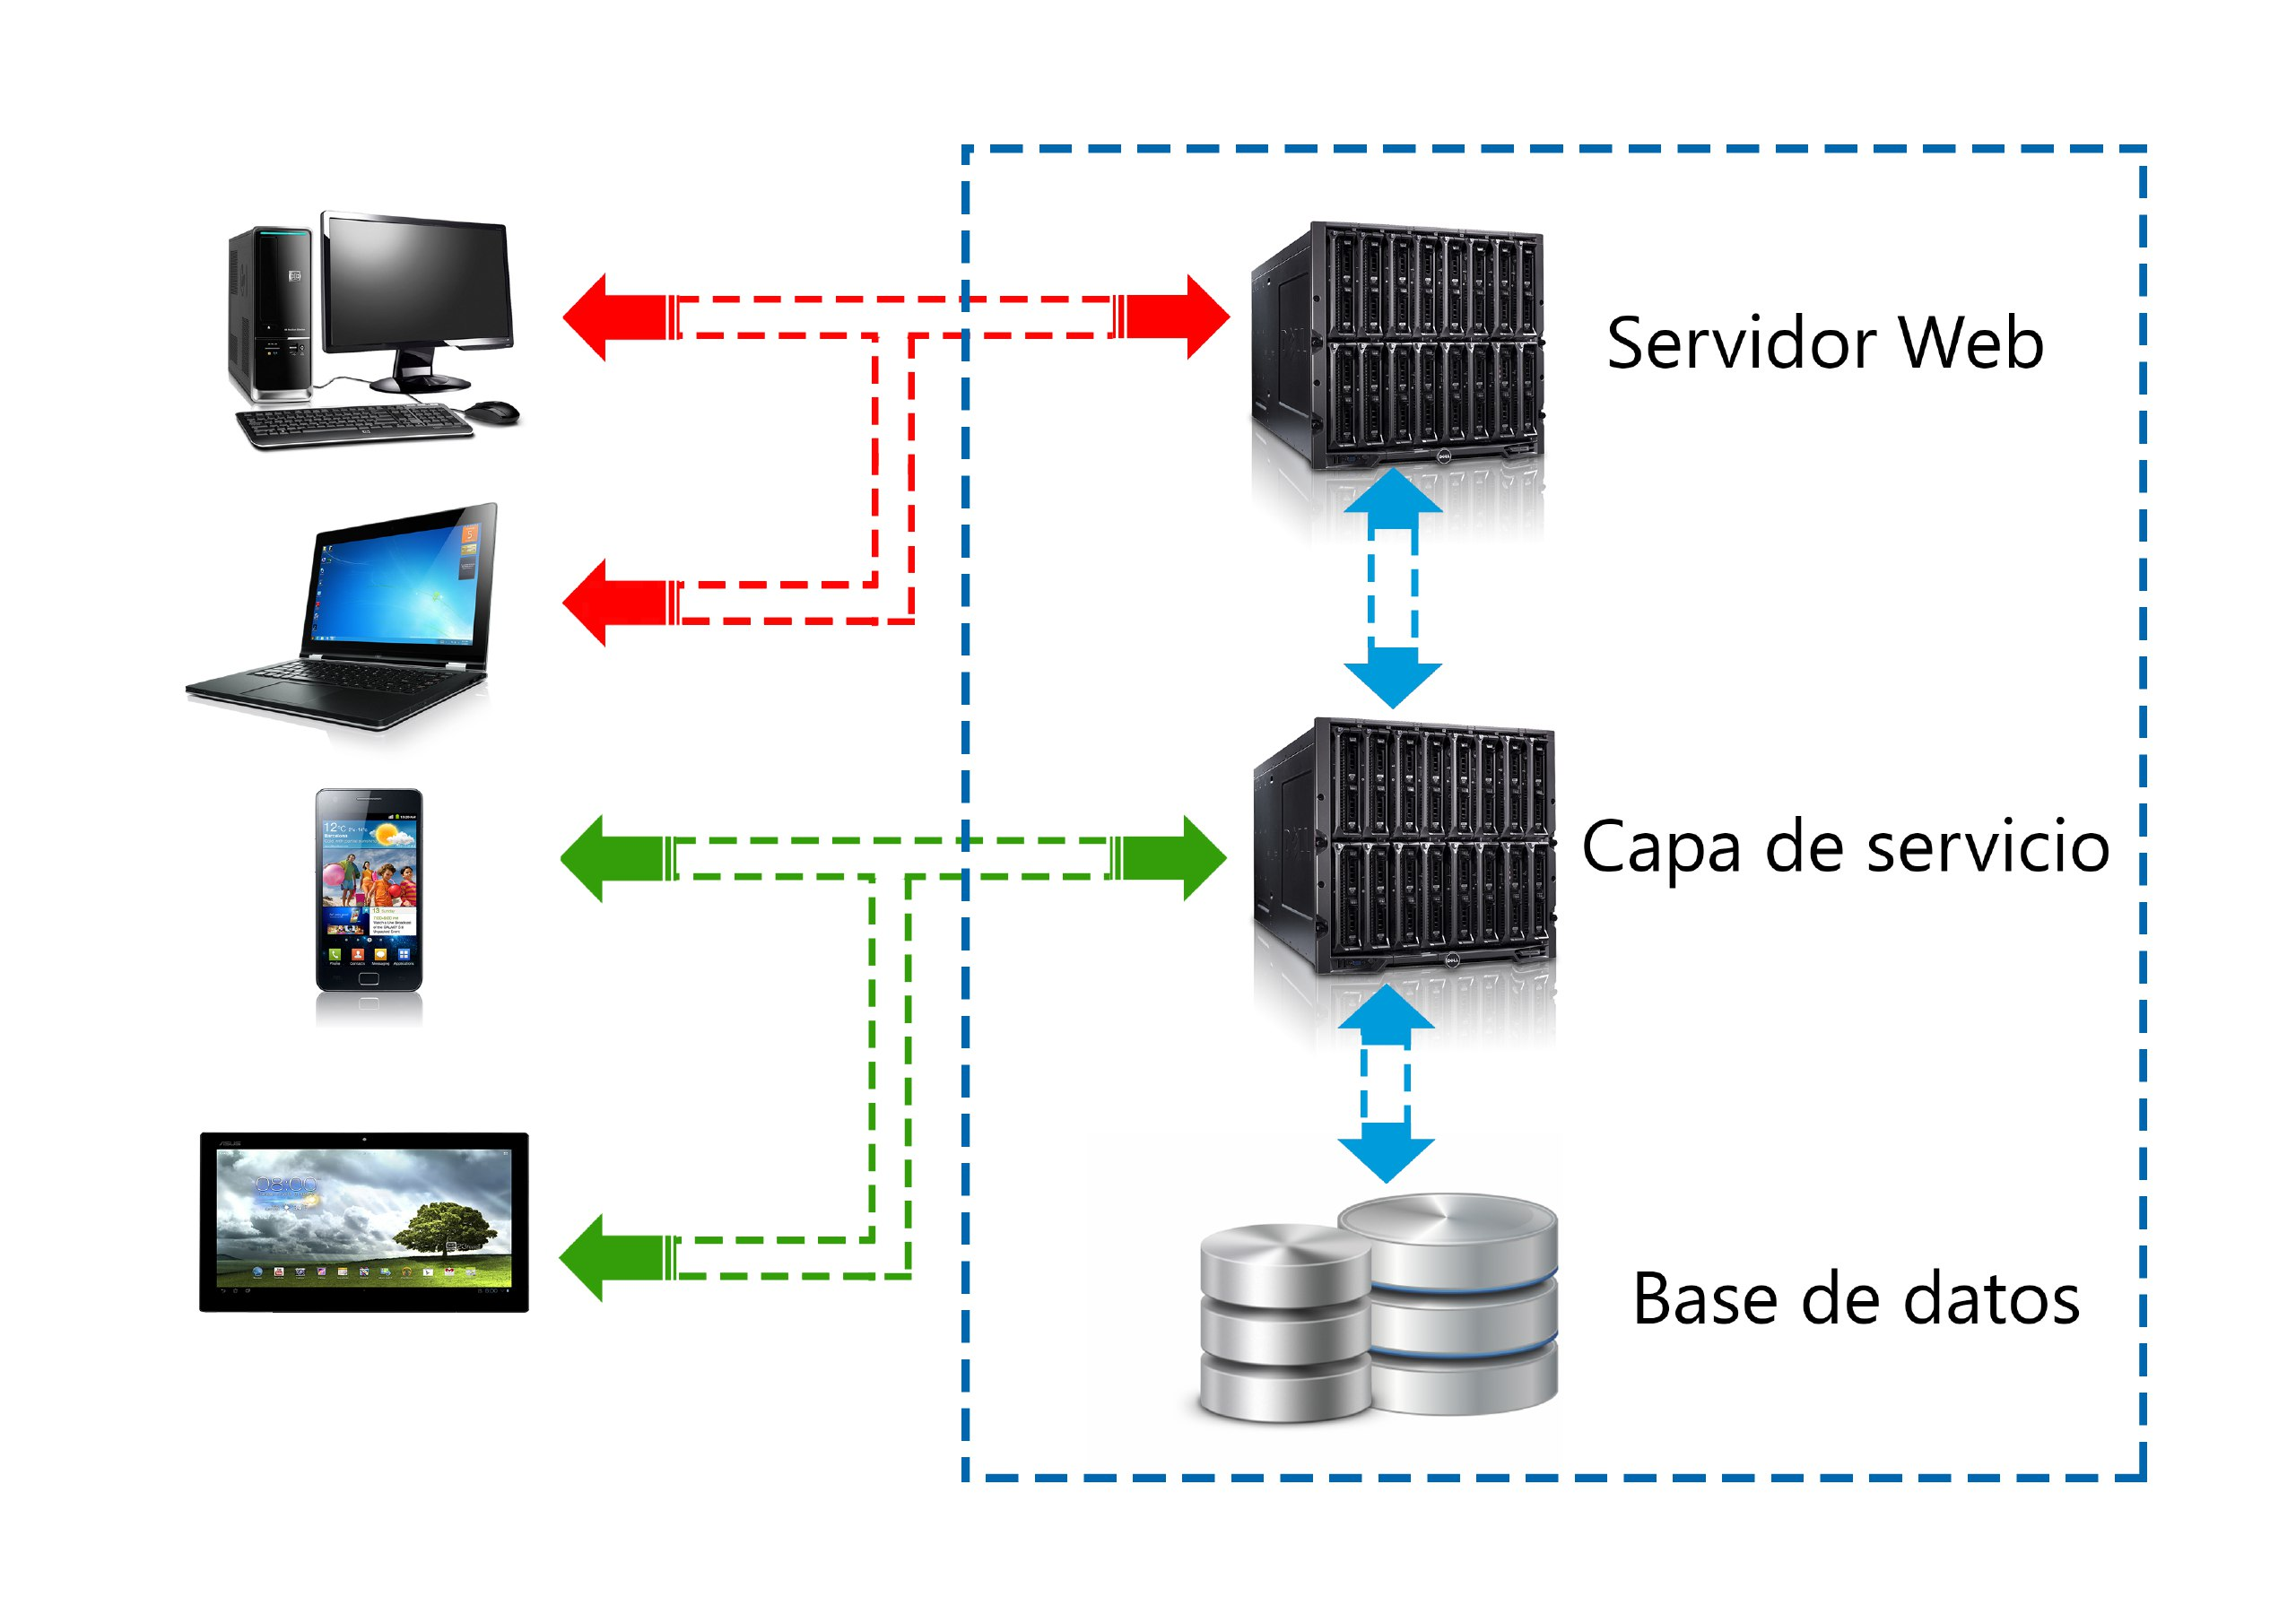
\includegraphics[width=.8\textwidth]{img/tp1_integrador/arquitectura_del_sistema}
  \caption{Arquitectura del sistema}
  \label{arquitectura}
\end{figure}

\item \textbf{Capacitación e instrucciones de uso}:

Se realizarán videos para explicar el funcionamiento del sistema desde el punto de vista del paciente  y otro desde el punto de vista del médico, dichos videos se publicarán en la página oficial de nuestro sistema y en Youtube.

Se añadirán mensajes de ayuda en la misma vista que permita al usuario comprender todas y cada una de las opciones. Esto se implementara con un asistente de iniciación interactiva que le permite al usuario que ingresa por primera vez conocer cuales son las funcionalidades que brinda el sistema. Además se hará uso de la opción ayuda que le permita al usuario poder encontrar rápidamente lo que está buscando y explotar la máximo las funcionalidades otorgadas.

El manual de usuario incluirá las siguientes secciones
\begin{itemize}
\item   Una página de portada.
\item   Una página de título.
\item   Una página de derechos de autor.
\item   Un prefacio, que contiene detalles de los documentos relacionados y la información sobre cómo navegar por la guía del usuario.
\item   Una página de contenido.
\item   Una guía sobre cómo utilizar al menos las principales funciones del sistema, es decir, sus funciones básicas.
\item   Una sección de solución de problemas que detalla los posibles errores o problemas que pueden surgir, junto con la forma de solucionarlos.
\item   Una sección de preguntas frecuentes.
\item   Dónde encontrar más ayuda, y datos de contacto.
\item   Un Glosario y, para documentos más grandes, un Índice.

\end{itemize}

\item \textbf{Publicidad y propaganda}:

Antes de comenzar a definir que técnicas utilizaremos, es necesario diferenciar a estos dos métodos. Por un lado, la publicidad es una herramienta que se utiliza con objetivos comerciales; en nuestro caso conseguir una venta. La propaganda por otro lado difiere de la publicidad, su objetivo es modificar ideologías, costumbres y la visión de la realidad, objetivo fundamental de nuestro sistema.

Invertiremos en realizar publicidad en aquellos sitios web de salud que lo permitan, para conquistar a aquellos usuarios interesados por su cuidado personal.

Utilizaremos lugares relacionados a la salud para dar a conocer nuestro producto, estos lugares pueden ser hospitales, farmacias, centros de salud, etc. Aprovecharemos la intima relación que tiene nuestro sistema con los lugares antes citados para establecer  convenios que permitan el beneficio mutuo  a partir de la prestación del servicio de nuestro sistema. 
Por ejemplo actualmente existen farmacias que brindan, a sus clientes, la posibilidad  de acceder a una cuenta para ver  los productos que se ha comprado a lo largo de su historia como cliente, dándoles puntos por cada compra que luego podrán canjear, sería interesante ofrecerle a esas farmacias nuestro sistema para que ellos le brinden a sus clientes mas beneficios y así nuestro sistema se beneficiaría con la popularidad del mismo.

También será necesario realizar una buena campaña de marketing utilizando propaganda en Youtube para atrapar a aquellos usuarios que no se encuentran familiarizados con la tecnología, pero que si se interesarán por los beneficios que ofrece nuestro sistema.
\end{enumerate}


\begin{comment}
http://velneo.es/cual-es-la-mejor-forma-de-vender-software-a-empresas-de-un-sector-especializado/
http://velneo.es/como-vender-programas-de-software/
http://velneo.es/segmentacion-de-mercado-en-software/
http://une-senn.tripod.com/new_page_3.htm
http://asistemgrp5.weebly.com/plan-de-conversioacuten.html
Método de conversión o implementación: directa, en paralelo, piloto, pruebas de versiones

Actividades: como hacer la publicidad, la promoción, como linquearlo, capacitación pilóto,  migracion de base de datos, configuración y diseño de red,
______________________________________________________________
Método de conversión del sistema, metodos, actividades y justificaciones. Siempre hay un sistema del que partimos, siempre hay una conversión de lo antiguo a lo actual. Directa, en paralelo, piloto.
Capacitación puede ser. Nuestro desafío es que la gente está muy encasillada en como se maneja con la salud, tenemos que ver como se lo vamos a hacer entrar. Antes la gente guardaba sus documentos de salud en un armario.
\end{comment}

\newpage

\subsection{Negociación}

\subsubsection{Introducción}

Se debe elaborar una guía de temas o aspectos a tener en cuenta y la estrategia para ir a negociar con un directivo del Cliente. Los temas a negociar serán: Cómo se cumplirán las expectativas del Cliente, la aprobación para el inicio del proyecto, cantidad de tiempo, cómo se organizará el trabajo, precios, gastos. 


%Los temas a tratar serán los siguientes :
\subsubsection{Guía de temas a tratar con el cliente}
\begin{itemize}
\item Expectativas del cliente
	\begin{itemize}
		\item Aspectos de rendimiento de consultas y respuestas al sistema
		\item Interfaz de usuario
		\item Accesibilidad
        \item Usabilidad
		\item Riesgos
	\end{itemize}
\item Planificación
	\begin{itemize}
		\item Duración de etapas
        \item Entregables
        \item Recursos humanos temporales
        \item Hardware específico
	\end{itemize}
\item Equipos de trabajo
	\begin{itemize}
		\item Nomina de personal afectada
		\item Asistencia técnica/Mesa de Ayuda
	\end{itemize}
\item Presupuesto
	\begin{itemize}
		\item Detalle de gastos
		\item Cronograma de erogación
	\end{itemize}
\item Inicio del proyecto
	\begin{itemize}
		\item Hitos
		\item Etapas
		\item Firma del contrato
	\end{itemize}
\end{itemize}

\subsubsection{Conducción de la negociación}
\begin{itemize}
	\item Premisas
		\begin{itemize}
			\item Asistir con vestimenta adecuada
			\item Ser puntual
			\item Mantener un tono amable y cordial así como un lenguaje sencillo
		\end{itemize}
    
	\item Aspectos relevantes de cada tema de la negociación
    \begin{itemize}
		\item Expectativas del cliente
		\begin{itemize} 
			\item Esbozar las bondades de la plataforma propuesta en forma sintética no más de dos minutos. Repaso de funcionalidades acordadas y los objetivos de cada una.
			\item Hacer hincapié en que serán desarrolladas interfaces intuitivas para facilitar el uso del sistema al usuario.
			\item Exponer en forma sencilla aspectos técnicos de infraestructura:
			\begin{itemize}
				\item Enlace: Este término englobará a muy alto nivel cualquier aspecto técnico relacionado con las conexiones de datos.
				\item Sistema: Este término englobará todas las funcionalidades previstas.
				\item Servidores: Este término englobará los servicios prestados a través del enlace (Base de Datos, Web, Respaldo).
			\end{itemize}
            \item Enunciar riesgos principales del proyecto. Advertir sobre la posible variación de costos en relación al proceso inflacionario.
		\end{itemize}
        
		\item Inicio de Proyecto
        
	    \begin{itemize}
			\item Informar las etapas del proyecto, repasando brevemente las actividades principales de cada una, mencionando solamente las actividades relevantes.
			\item Estas actividades relevantes serán aquellas que interactúan directamente con el cliente.
			\item Fecha de inicio: Sugerir al cliente una fecha de inicio que no superponga al proyecto a desarrollar con los que estén finalizando. Asegurarle que el valor del proyecto no va a cambiar sustancialmente hasta esa fecha de inicio.
			\item Repasar los aspectos principales del contrato y luego firmarlo.
        \end{itemize}
        
		\item Planificación.
        
		\begin{itemize}
			\item Informar de la planificación al cliente, evitar disuadir al cliente de realizar modificaciones en las fechas de entrega, indicándole que los costos podrían cambiar con las modificaciones de las fechas.
	    \end{itemize}
        
		\item Equipo de Trabajo
        
    	\begin{itemize}
			\item Informar al cliente según el cronograma del proyecto, cuales son los equipos que van a intervenir en el desarrollo, en que fechas se reunirán con él, además de dar la nómina de referentes de cada equipo.
			\item Hacer mención de los referentes de Atención al cliente/Mesa de ayuda como vínculo directo para asistir cualquier consulta o resolver cualquier problema.
		\end{itemize}
        
		\item Presupuesto
        
	    \begin{itemize}
			\item Repasar el detalle de ítems del proyecto y su costo
			\item Negociar formas de pago y cronograma de desembolsos
		\end{itemize}
	\end{itemize}
\end{itemize}


\subsubsection{Tips para situaciones complejas}

\begin{itemize}
	\item Expectativas del cliente:	Se esbozarán las ventajas del nuevo sistema centrandonos en las características esenciales solicitadas por el cliente y explicando con el Líder técnico los métodos de resolución de los problemas complejos.
    
	Debemos destacar que es esencial la participación del usuario tanto al momento de capturar requisitos como en cualquier otro momento del desarrollo para garantizar un producto de soporte pleno a las actividades de la organización.
    El sistema logrará esto a través del uso de las tecnologías de información de vanguardia ofreciendo la realización de tareas, la disponibilidad,gestión y el intercambio de datos.
    \begin{itemize}
		\item Aspectos de rendimiento de consultas y respuestas al sistema: se le informará al usuario que el rendimiento del sistema podrá sufrir fluctuaciones debido a la red subyacente e Internet.
No se realizaran aseveraciones sobre tiempos de respuestas específicos.

		\item Interfaz de usuario: Acompañaremos la entrevista con prototipos de interfaces de usuario, de esta manera le transimitiremos al cliente de mejor manera nuestra visión del sistema terminado y se familiarizará con el look \& feel de la misma.

		\item Accesibilidad: Se le informará al cliente bajo que condiciones el sistema se encontrará accesible.
        Esto implica acordar con el cliente que, el sistema, ante determinados eventos de la red, o del servidor se puede encontrar inaccesible temporalmente.
        
        \item Usabilidad: facilidad con que los usuarios podrán utilizar el sistema, cómo van a interactuar con el sistema, como el sistema va a responder a las acciones ejecutadas por el usuario, cuan intuitivo será su desenvolvimiento en el mismo.

		\item Riesgos: se le informará al cliente, los riesgos vinculado a la disponibilidad del servicio en la Internet (posibles ataques),se informará sobre el marco de cobertura contra intrusiones y daños del sistema, comentaremos que nuestro sistema contará con sistemas RAID, para evitar la perdida de datos y con sistemas de control de versiones sobre registros con expiración lo que permitirá deshacer cambios por parte de los usuario, y no perder datos de la BD inmediatamente son borrados.
	\end{itemize}

Las cuestiones previamente nombradas serán desarrolladas intentando despejar cualquier tipo de dudas por parte del negociador.
En caso de que este no cuente con la información técnica solicitada por el cliente el personal técnico que lo acompañe podrá participar.
El lenguaje corporal deberá mostrar seguridad para expresar los términos de negociación. 
Se deberá mantener una relación cordial, siempre manteniendo el mismo tono de voz, sin cruzar los brazos o piernas.

	\item Planificación: Debemos tener en cuenta que el cliente tiene una visión del proyecto a desarrollar, por lo que puede haber hecho averiguaciones sobre los tiempos de desarrollo.
Pero nuestro experiencia liderando proyectos previos y nuestra formación académica nos han brindado métodos para calcular los tiempos con mucha precisión.
Si el cliente intenta acortar los tiempos deberemos remarcar que los tiempos informados tienen un breve margen de holgura para contener imprevistos, por lo cual acortar el proyecto puede impactar negativamente en sobre la gestión de riesgos en el proyecto, aumentando las probabilidades de entregar un software incompleto y con errores.
Lo cual no estamos dispuestos a realizar, debido a que nuestra política es entregar software de alta calidad a nuestros clientes y somos reconocidos en el mercado por este hecho.
Si el cliente insistiese habría que disuadirlo para que cambie de opinión.
Enfocandonos en que la supresión de funcionalidades o en hacer hincapié en que los tiempos que se puedan cambiar no afectaran sustancialmente los costos del proyecto.
	\begin{itemize}
		\item Duración de etapas: El proyecto estará organizado en etapas denominadas sprints, los cuales tendrán una duración de 22 días en donde se desarrollara un incremento "terminado" y potencialmente desplegable del producto. Cada una dividida en subetapas (Análisis, Diseño, Implementación, Prueba).
        \item Entregables: funcionalidades, junto con su código y manuales que explican el correcto uso de la porción de funcionalidad entregada.
        \item Recursos humanos temporales: se definirán las etapas críticas del proyecto en las cuáles se podrá recurrir al outourcing para la finalización a tiempo de la misma.
        \item Hardware específico: con el tiempo se estima que el proyecto escale y sea necesario la incorporación de hardware específico y complejo, se establecerá los posibles recursos que se estima puedan llegar a ser de suma necesidad con el crecimiento del proyecto.
	\end{itemize}
    
	\item Equipos de trabajo: El cliente debe estar informado acerca de que se necesitará interactuar con personal de la empresa que actualmente hace uso del sistema antiguo e incluso con el mismo, además de que necesitaremos de una persona perteneciente a su empresa con la que podamos tener contacto constante y nos pueda quitar dudas acerca de diferentes temas relacionados al conocimiento de la empresa y su sistema antiguo para que desarrolle el papel del Product Owner.
Además se hará hincapié en la formación académica de nuestro personal y en la envergadura de los proyectos sobre los que han trabajado para que el cliente sienta seguridad sobre la privacidad de sus datos, además de aportarle al crecimiento de su organización.

	\begin{itemize}
		\item Nomina de personal afectado: ver anexo \ref{nomina}
%NOMINA DEL PERSONAL AFECTADO
		\item Es importante hacer notar al cliente que contamos con personal para informarle en que estado se encuentra el Proyecto, y qué podrá consultar cualquier tipo de problemática o duda con nuestro personal respecto a la evolución del mismo.

	\end{itemize} 
 
	\item Presupuesto
    En este punto quizás notemos que la visión del cliente sobre los costos es muy reducida.
Se le deben hacer notar con mucha amabilidad que aunque el software es un producto intangible, este cuenta con muchas horas hombre detrás, además de requerir personal capacitado, haciendole notar la calidad con la que contamos contrastandolo con el faltante de mano de obra calificada en el mercado. 
En ningún momento se le dará información sobre la estructura de costos de la empresa que generan los valores del presupuesto.

	\begin{itemize}
		\item Detalle de gastos:
        Aunque los costos estén desglosados por las etapas previamente nombradas, se le deberá aclarar al cliente que el sistema es un Todo, por lo que es inaceptable contratarlo parcialmente, solicitando algunas de las partes.
Esto de nuevo tiene que ver con la calidad de los sistemas que entregamos.

		\item Cronograma de erogación:
        Los desembolsos serán realizados en 3 partes iguales, del precio total del producto las mismas fueron estipuladas en base a su necesidad para el correcto desempeño del procesos de realización del sistema, por lo que serán fechas inamovibles para el cumplimiento con las fechas estipuladas en el contrato.
Ver anexo \ref{contrato} correspondiente al mismo.
	\end{itemize}
    
    
En este tipo de reuniones no se deben tratar aspectos técnicos propios de la implementación, se deben evacuar dudas en un grado conceptual.
No se debe nunca llegar al choque. 
El representante debe actuar como moderador, dándole continuidad al hilo principal de la reunión.
Se estructurará la reunión para que no se exceda de una hora y esto será informado al cliente (preparándonos para que se extienda unos 20 minutos mas).
Se irá a la reunión con un primer contrato para revisar por parte del cliente sobre el que se harán las modificaciones necesarias señaladas por el cliente, siempre que las mismas no vayan en contra de lo expresado anteriormente.

	\item Inicio del Proyecto
    Debemos repasar los hitos especificados en el contrato así como las etapas que hemos definido. 
    El negociador explicará como esta formulado el mismo y le detallará al cliente en que partes del contrato esta lo que se ha conversado durante el transcurso de la reunión.
    En caso de haber acordado algún cambio se coordinara una nueva reunión con el cliente.
    El contrato se puede ver en el anexo \ref{contrato} y en el anexo \ref{contrato2} podemos encontrar un sistema alternativo sin desarrollo del Front-End (Ya que el cliente podría haber solicitado este tipo de sistema y que el sector de sistemas de su empresa le desarrolle el Front-End).
\end{itemize}
